% VERSTERKER

    In dit verslag wordt het designproces van hoogfrequente single-stage
    versterker besproken die gerealiseerd wordt in common emitter-opstelling.

    Hierbij is de gebruikte NPN-transistor een BFR91A en werd
    het werkingspunt in \cite{lesWendy} gespecificeerd zoals weergegeven in
    \autoref{tbl:OPSpec}.
      \begin{table}[h!]
        \begin{center}

        \caption{DC werkingspunt transistor}
        \label{tbl:OPSpec}
        
 \begin{tabular}{|l|l|l|l|} 
\hline \textbf{Groep} & \textbf{Frequentie $f_0$} & \textbf{$V_{ce}$} & \textbf{$I_c$}\\ 
\hline $1$ & $1445$ MHz & $5$ V & $5$ mA \\ 
\hline \end{tabular} 

        \end{center}
      \end{table} 
    
    Voor deze werkingsfrequentie werden de $S$-parameters gegeven in \cite{lesWendy}:
    \[
S = \left[ \begin{array}{cc} 
S_{11} & S_{12} \\ 
 S_{21} & S_{22} \\ 
\end{array} \right] 
 \approx \left[ \begin{array}{cc} 
-0.104 +0.181 j & 0.102 +0.154 j \\ 
1.369 +1.397 j & 0.355 -0.318 j \\ 
\end{array} \right] \label{eq:S}
\]
    
\section{Stabiliteit}
  
    We controleren de nodige en voldoende voorwaarde voor stabiliteit van de versterker
    door middel van formules 11.71 en 11.72 van \cite{Pozar}.
    Dit is het Rollet-stabiliteitscriterium.
    \[
      K = \frac{1 - \left| S_{11} \right|^2 - \left| S_{22} \right|^2 + \left| \Delta \right|^2}{2 \left| S_{12}S_{21} \right|} > 1
    \]
    \[
      \left| \Delta \right| < 1
    \]
    \[
      \Delta = \det{S} = S_{11}S_{22} - S_{12}S_{21}
    \]
    
    Aan deze voorwaarden is voldaan, zodat we kunnen besluiten dat de te realiseren versterker onconditioneel stabiel is.
  \section{Stabiliteitscirkels}
    Vermits de versterker onconditioneel stabiel is, zullen de stabiliteitscirkels
    ofwel de volledige Smith Chart omvatten ofwel buiten de Smith Chart vallen.
    \tbd{BESPRE CIRKEL = 1}
    Met formules 11.68 en 11.69 uit \cite{Pozar}, worden middelpunt $C$ en
    straal $R$ van de stabiliteitscirkels bepaald.
    \[
      C_L = \frac{\conj{\left(S_{22} - \Delta \conj{S_{11}}\right)}}{\left| S_{22} \right|^2 - \left|\Delta\right|^2}
      \qquad \qquad \qquad
      R_L = \left| \frac{S_{12}S_{21}}{\left| S_{22} \right|^2 - \left|\Delta\right|^2}\right|
    \]
    \[
      C_S = \frac{\conj{\left(S_{11} - \Delta \conj{S_{22}}\right)}}{\left| S_{11} \right|^2 - \left|\Delta\right|^2}
      \qquad \qquad \qquad
      R_S = \left| \frac{S_{12}S_{21}}{\left| S_{11} \right|^2 - \left|\Delta\right|^2}\right|
    \]
    Dit geeft aanleiding tot volgende waarden:
    \[
	C_L =	  2.70 + j   2.15\qquad \qquad \qquad  	R_L =	  2.37
\]

    \[
	C_S =	  7.04  +7.73 j\qquad \qquad \qquad	R_S =	 11.58
\]

    Op \autoref{fig:stabCirkels} kunnen deze cirkels ge\"inspecteerd worden.
    \begin{figure}[!h]
      \centering
      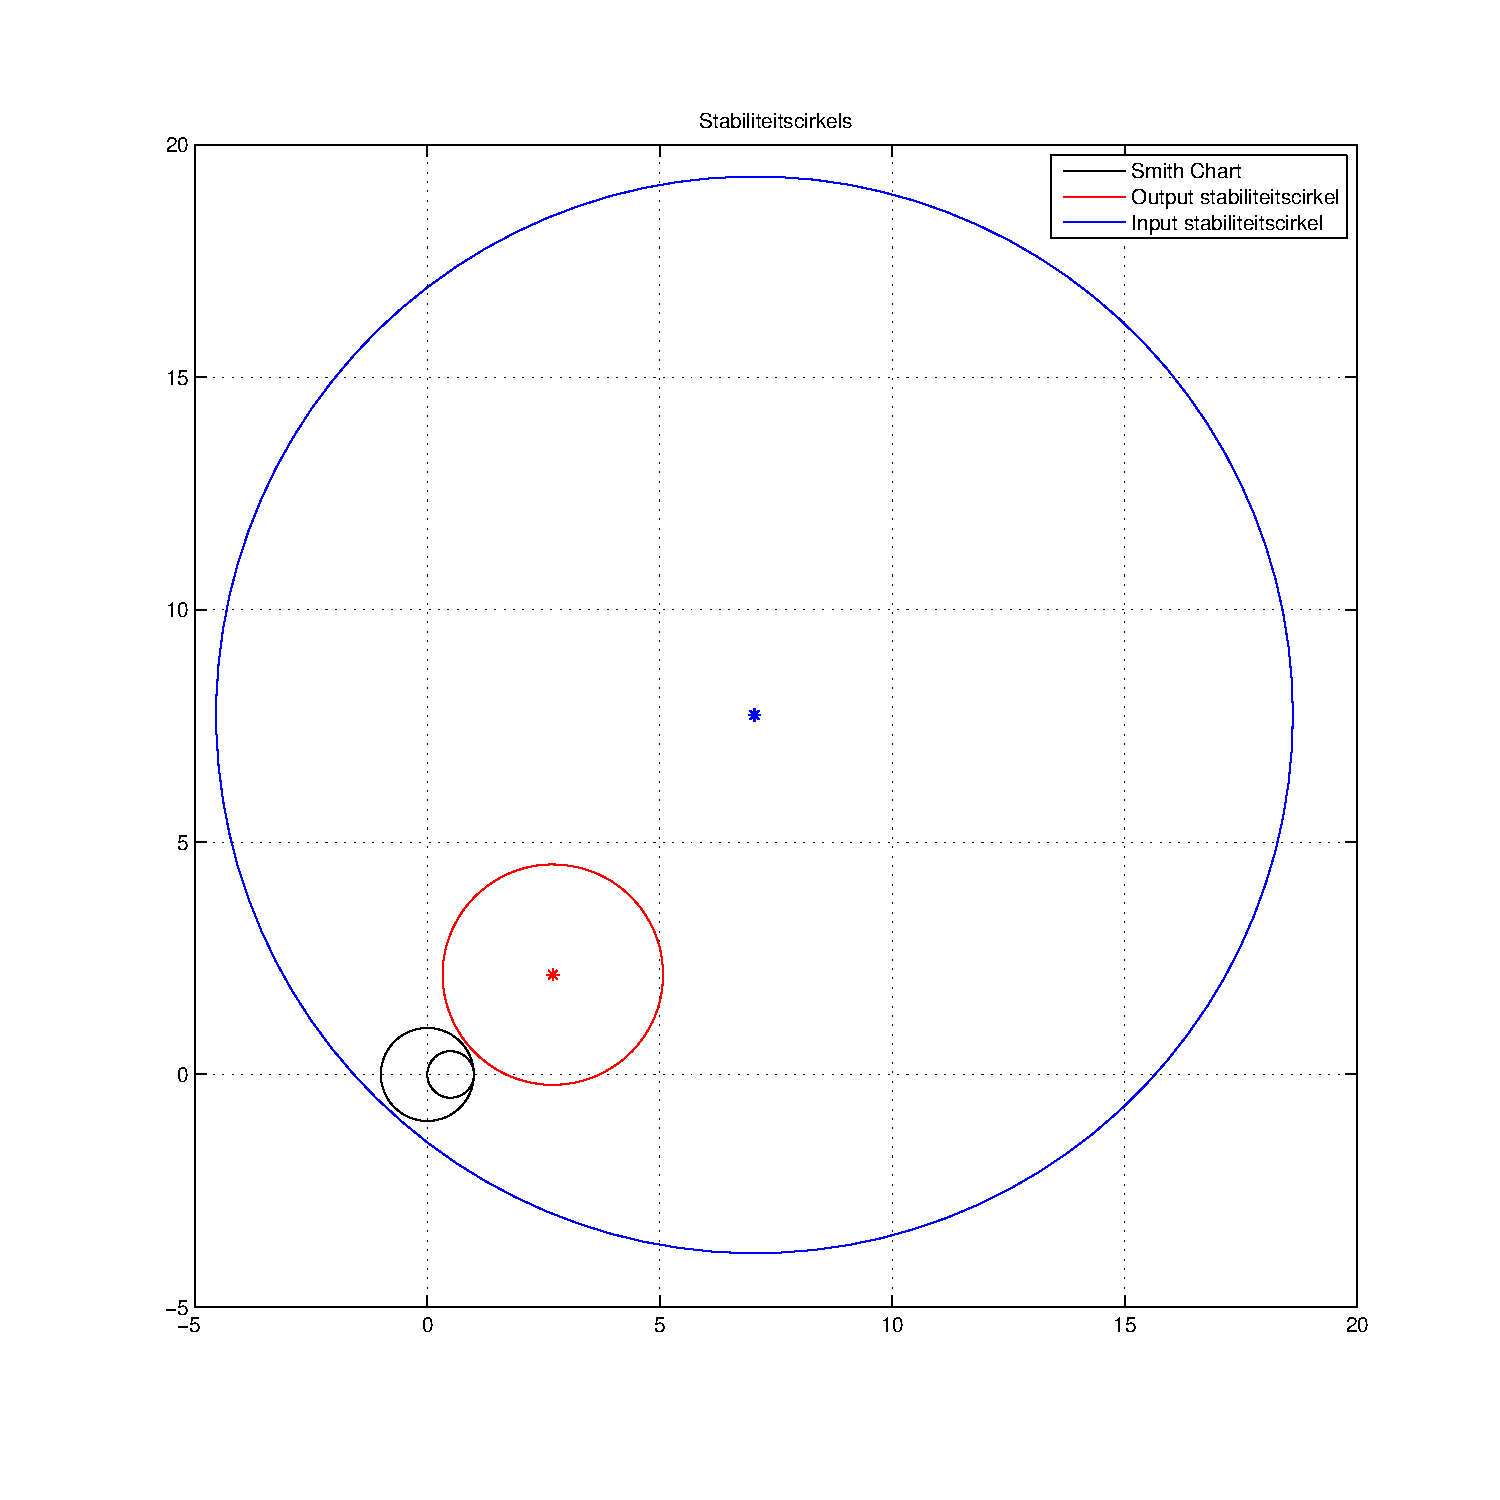
\includegraphics[width=\textwidth,keepaspectratio=true]{fig/stabiliteitscirkels.pdf}  
      \caption{Stabiliteitscirkels} 
      \label{fig:stabCirkels}
    \end{figure}
    Als extra controle, bekijken we welke zones van de Smith Chart stabiel zijn voor input en output. We volgen hier
    een analoge redenering als beschreven op pagina 614 van \cite{Pozar}.
    
    \paragraph{Voor de input} weten we dat indien de output perfect gematcht is
    ($Z_L = Z_0$ en dus ook $\Gamma_L = 0$, oftewel in het midden van de Smith
    Chart), we formule 11.62a uit \cite{Pozar}
    \[
      \left| \Gamma_{in} \right| = \left| S_{11} + \frac{S_{12}S_{21}\Gamma_L}{1 - S_{22}\Gamma_L} \right| < 1
    \]
    kunnen vereenvoudigen tot:
    \[
      \left| S_{11} \right|  < 1
    \]
    als voorwaarde voor stabiliteit. Hieraan is voldaan zoals we kunnen zien uit
    de S-parameters van de transistor. Hierdoor weten we dat het gebied binnen
    de blauwe inputsstabiliteitcirkel stabiel is.
    
    \paragraph{Voor de output} volgt analoog dat indien de input perfect
    gematcht is ($Z_S = Z_0$ en dus ook $\Gamma_S = 0$, oftewel in het
    midden van de Smith Chart), we formule 11.62b uit \cite{Pozar}
    \[
      \left| \Gamma_{out} \right| = \left| S_{22} + \frac{S_{12}S_{21}\Gamma_S}{1 - S_{11}\Gamma_S} \right| < 1
    \]
    kunnen vereenvoudigen tot:
    \[
      \left| S_{22} \right|  < 1
    \]
    als voorwaarde voor stabiliteit. Hieraan is voldaan zoals we kunnen zien uit
    de S-parameters van de transistor. Hierdoor weten we dat het gebied buiten
    de rode outputsstabiliteitcirkel stabiel is.
    

\section{Gebruik van de unilaterale benadering}
  Als verantwoording voor de unilaterale benadering, gebruiken we formule 11.86
  uit \cite{Pozar} die slechts enkele tienden van een dB afwijking mag geven.
  We nemen hiervoor de grenswaarde van $0.8 dB$
  \[
    -0.8 dB < \frac{1}{\left( 1 + U\right)^ 2} < \frac{G_T}{G_{TU}} < \frac{1}{\left( 1 - U\right)^ 2} < 0.8 dB
  \]
  In deze formule is $U$ de \textit{unilateral figure of merit}:
  \[
    U = \frac{\norm{S_{12}} \norm{S_{21}} \norm{S_{11}} \norm{S_{22}}}{ \left( 1 - \norm{S_{11}}^2 \right) \left( 1 - \norm{S_{22}}^2 \right)}
  \]
  In numerieke waarden, geven deze vergelijkingen dus:
    \[
	U \approx	0.04863
\]
\[
-0.8 \,dB < 0.90940 < \frac{G_T}{G_{TU}} < 1.10484 < 0.8 \,dB
\]
\[
-0.8 dB < -0.825 \,dB< \frac{G_T}{G_{TU}} < 0.866 \,dB< 0.8 \,dB
\]

  Vermits deze ongelijkheden ongeldig zijn, gebruiken we de bilaterale vormen.
  Maar vermits deze waarden niet te veel afwijken, zal een unilaterale
  benadering geen totaal foute waarden geven.
  
  

\section{Berekening van maximale versterking}
  Aan de hand van \cite{Pozar} en \cite{Gonzalez} bepalen we de maximale
  versterking die mogelijk is met deze transistor voor
  de opgegeven werkingsfrequentie.
  
  In appendix E van \cite{Gonzalez} werd bewezen dat bovenstaande uitdrukking
  voor een onconditioneel stabiele transistor (K > 1) en simultane input- en
  outputmatching, de maximale versterking uitgedukt
  kan worden als:
  \[
    G_{Tmax} = \frac{\norm{S_{21}}}{\norm{S_{12}}} \left( K - \sqrt{K^2-1}\right)
  \]
  
  
  \section{Bepaling van de constante gaincirkels}
  Uit formules 5.96 en 5.100 van \cite{lessen} kunnen we het middelpunt en de
  straal van de constante gaincirkels voor gain $G_p$ bepalen.
  \[
    C = \frac{\left( \conj{S_{22}} - S_{11} \conj{\Delta} \right)}{\norm{S_{22}}^2 - \norm{\Delta}^2 + \frac{\norm{S_{21}}^ 2}{G_p}}
  \]
  \[
    R = \frac{\sqrt{\norm{S_{12} S_{21}}^2 - 2 K \norm{S_{12} S_{21} \frac{\norm{S_{21}}^2}{G_p} + \frac{\norm{S_{21}}^2}{G_p} }}}{\norm{S_{22}}^2 - \norm{\Delta}^2 + \frac{\norm{S_{21}}^2}{G_p}}
  \]
  Voor een versterking van enkele verschillende versterkingen $G_p$ bekomen we
  in deze formule de waarden weergegeven in \autoref{tbl:gainCirkels}.
    \begin{table}[h!]
    \begin{center}
    \caption{Constante gaincirkels}
    \label{tbl:gainCirkels}
    \begin{tabular}{|r|r|r|} \hline 
\textbf{Versterking $G_p$} & \textbf{Middelpunt $C$} & \textbf{Straal $R$} \\ \hline 
$ 3.000$ \mbox{dB} & $ 0.111 -0.127 j$ &  0.804 \\ \hline 
$ 2.000$ \mbox{dB} & $ 0.100 -0.113 j$ &  0.824 \\ \hline 
$ 1.000$ \mbox{dB} & $ 0.089 -0.102 j$ &  0.843 \\ \hline 
$10.390$ \mbox{dB} & $ 0.243 -0.277 j$ &  0.561 \\ \hline 
$16.323$ \mbox{dB} & $ 0.433 -0.492 j$ &  0.062 \\ \hline 
$16.411$ \mbox{dB} & $ 0.436 -0.495 j$ &  0.000 \\ \hline 
\end{tabular}
    \end{center}
    \end{table}
  
  Op de Smith Chart \cite{smithchart} in \autoref{fig:gainCirkels} worden deze
  constante gain cirkels voor enkele verschillende
  versterkingen weergegeven op.
  \begin{figure}[!h]
      \centering
      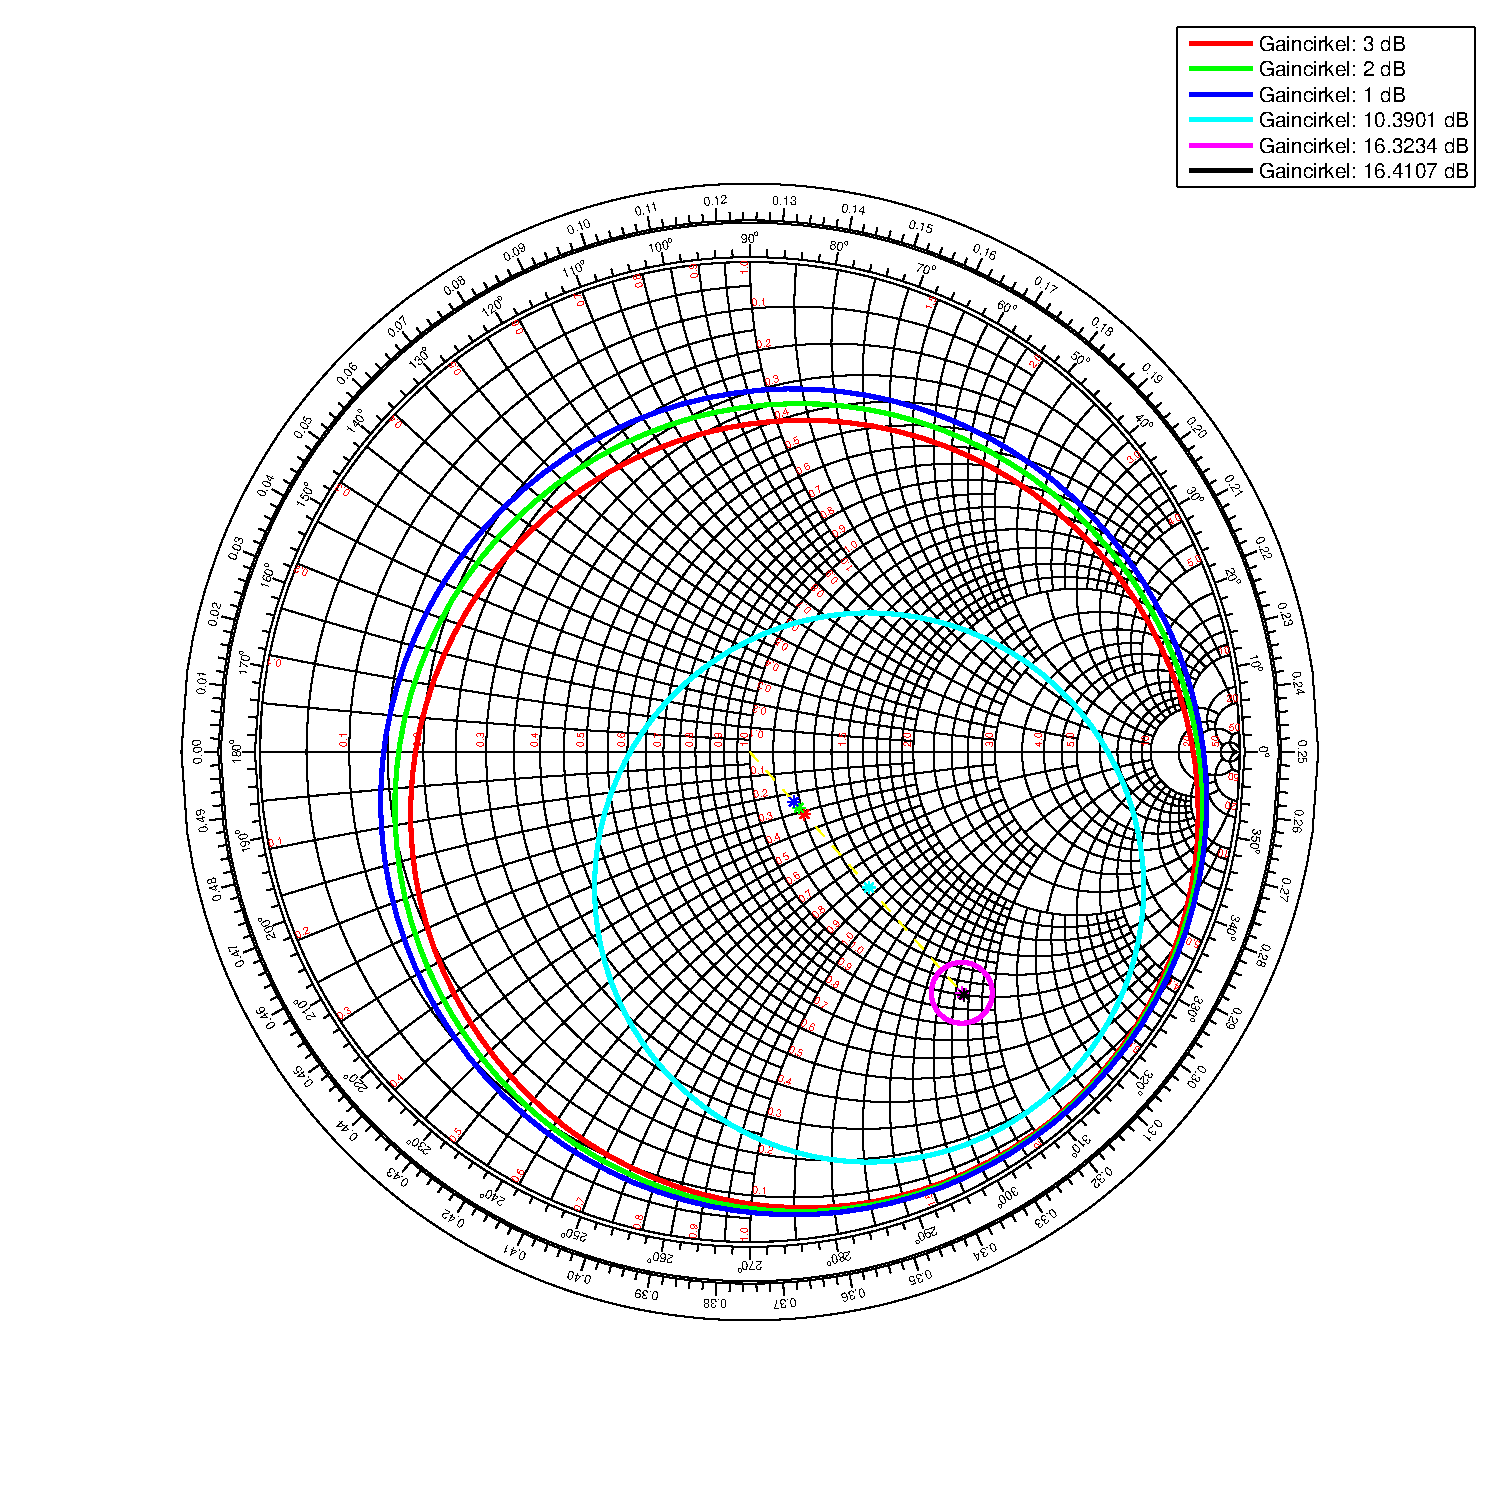
\includegraphics[width=\textwidth,keepaspectratio=true]{fig/gaincirkels.pdf}  
      \caption{Constante gaincirkels} 
      \label{fig:gainCirkels}
    \end{figure}
  

\section{Matchingnetwerken}

\section{DC biasnetwerk}
  Om het DC Bias-netwerk te designen maken we gebruik van \cite{Gonzalez}

\section{Simulaties}
  \subsection{Ideale transmissielijnen}
  \subsection{Microstrip}

\section{Lay-out}

\section{Metingen}
\subsection{Vergelijking metingen en simulaties}




\tbd{\textbf{Voor het verslag:}
  \begin{itemize}
    \item Alle berekeningen + verwijzing formule
    \item Plots van ideale simulaties + simulatie in microstripversie
    \item Gebruikte Smith Charts voor matching van in- en uitgang
  \end{itemize}
  }